\documentclass[aspectratio=169,9pt]{beamer}
% Beamer layout
\setbeamersize{text margin left=0.4cm, text margin right=0.2cm}

% Math & fonts
\usepackage{amsmath,amssymb}
\usepackage{mathpazo}   % Palatino text + math

% Tables & units
\usepackage{booktabs}
\usepackage{siunitx}

% TikZ (one load, all libs)
\usepackage{tikz}
\usetikzlibrary{arrows.meta,calc,positioning,shapes.geometric,shapes.misc}

% Algorithms
\usepackage{algorithm}
\usepackage[noend]{algpseudocode}
\usepackage{float}

% Media
\usepackage{multimedia}
\usepackage{animate}

% Bibliography
\usepackage{natbib}


\newcommand{\shortdate}{\the\month-\the\day}
\graphicspath{{../../figures/.}}


\definecolor{cardinalred}{RGB}{140,21,21}
\definecolor{coolgray}{RGB}{77,79,83}
\definecolor{black}{RGB}{0,0,0}
\definecolor{beige}{RGB}{210,194,149}
\definecolor{darkbeige}{RGB}{179,153,93}
\definecolor{darkcardinal}{RGB}{94,48,50}
\definecolor{lightcardinal}{RGB}{141,60,30}
\definecolor{darkpurple}{RGB}{83,40,79}
\definecolor{darkcyan}{RGB}{0,124,146}
\definecolor{skyblue}{RGB}{0,152,219}
\definecolor{treegreen}{RGB}{0,155,118}
\definecolor{darkorange}{RGB}{168,101,12}
\definecolor{beigegray}{RGB}{95,87,79}
\definecolor{boxgray}{RGB}{238,235,233}
\definecolor{footergray}{RGB}{199,209,197}



\mode<presentation>

\setbeamercolor*{palette primary}{use=structure,fg=white,bg= cardinalred}
\setbeamercolor*{palette secondary}{use=structure,fg=white,bg= coolgray}
\setbeamercolor*{palette tertiary}{use=structure,fg=white,bg= darkcardinal}
\setbeamercolor*{palette quaternary}{fg=white,bg= darkbeige}

\setbeamercolor*{sidebar}{use=structure,bg= beige}
\setbeamercolor*{footer}{use=structure,bg= footergray,fg=darkcardinal}
  
\setbeamercolor*{palette sidebar primary}{use=structure,fg=structure.fg!10}
\setbeamercolor*{palette sidebar secondary}{fg=white}
\setbeamercolor*{palette sidebar tertiary}{use=structure,fg=structure.fg!50}
\setbeamercolor*{palette sidebar quaternary}{fg=white}

\setbeamercolor*{titlelike}{parent=palette primary}
\setbeamercolor*{foot line}{parent=palette secondary}

\setbeamercolor*{separation line}{}
\setbeamercolor*{fine separation line}{}

\setbeamercolor{itemize item}{fg=cardinalred}
\setbeamercolor{itemize subitem}{fg=cardinalred}
\setbeamercolor{itemize subsubitem}{fg=cardinalred}
\setbeamercolor{enumerate item}{fg=cardinalred}
\setbeamercolor{enumerate subitem}{fg=cardinalred}
\setbeamercolor{enumerate subsubitem}{fg=cardinalred}
\setbeamercolor{description item}{fg=cardinalred}

\setbeamertemplate{bibliography item}[text]
\setbeamertemplate{frametitle continuation}[from second]
\setbeamercolor{bibliography entry title}{fg=black}
\setbeamercolor{bibliography entry author}{fg=black}
\setbeamercolor*{bibliography entry location}{fg=black}
\setbeamercolor*{bibliography entry note}{fg=black}

\renewcommand*{\bibfont}{\small}
\setbeamertemplate{navigation symbols}{}

\setbeamerfont{footnote}{size=\tiny}

\mode
<all>
\definecolor{cardinalred}{RGB}{140,21,21}
%--- Custom footline
\setbeamertemplate{footline}{%
\begin{beamercolorbox}[wd=\paperwidth,ht=4ex,dp=2.5ex]{}
    \centering
    \makebox[0.32\paperwidth][l]{\scriptsize\texttt{Spec. \shortdate}}
    \makebox[0.32\paperwidth][c]{\scriptsize\texttt{$^{\dag}$masseyj@stanford.edu}}
    \makebox[0.32\paperwidth][r]{\scriptsize\insertframenumber/\inserttotalframenumber}
  \end{beamercolorbox}
}
\usepackage{algorithm}
\usepackage[noend]{algpseudocode}
\usetikzlibrary{arrows.meta,shapes.geometric,shapes.misc,positioning}

\tikzset{
  >={Stealth},
  proc/.style = {rectangle, rounded corners, draw, align=left, minimum height=8mm, text width=35mm, align=center},
  meas/.style    = {trapezium, trapezium left angle=70, trapezium right angle=110, draw, align=left, minimum height=8mm, text width=19mm, align=center},
  decision/.style = {diamond, aspect=2.2, draw, align=center, inner xsep=1.2ex, inner ysep=1ex, text width=2cm},
  smldec/.style = {diamond, aspect=2.2, draw, align=center, inner xsep=1.2ex, inner ysep=1ex, text width=19mm},
  terminator/.style = {ellipse, draw, align=center, minimum height=8mm, minimum width=16mm},
  line/.style  = {->, line width=0.6pt}
}


%--- Title info
\title{SU update: \\ Best estimate}
\author{JMO Massey$^{\dag}$, F Cabrera-Booman, JC Klewicki, T Jaroslawski, BJ McKeon}
\institute{Center for Turbulence Research \\ Stanford University}
% \thanks{This work was supported by DARPA under the CHAOS program}
\date{\today}

\begin{document}

%--- Title page
\begin{frame}
    \setcounter{framenumber}{0}
    \titlepage
    \vfill
    {\scriptsize \centering Thanks to DARPA for funding this work.\par}
\end{frame}

\begin{frame}

    \begin{itemize}
    %     \item Fix $U_e=14[\mathrm{m/s}]$
        \item $\delta\approx 0.035[\mathrm{m}]$, $U_e \approx14[\mathrm{m/s}]$, $T^+\equiv T u_\tau^2/\nu=10$
    \end{itemize}
    \begin{table}[]
        \centering
        \begin{tabular}{lccccc}
        \toprule
        Pressure (psi) & 0  &  50 & 100 \\
        \midrule
        $u_\tau$[m/s] & 0.58 & 0.47 & 0.52 \\
        $\nu/u_\tau$ [m] & 27$\times 10^{-6}$ & 7.5$\times 10^{-6}$ & 3.7$\times 10^{-6}$ \\
        $\nu$ [m$^2$/s] & 15.7$\times 10^{-6}$ & 3.52$\times 10^{-6}$ & 1.92$\times 10^{-6}$ \\
        $Re_\tau$ & 1,300 & 4,700 & 9,500 \\
        \textcolor{blue}{$f(T^+=10)$ [Hz]} & \textcolor{blue}{2,100} & \textcolor{blue}{4,700} & \textcolor{blue}{14,100} \\
        \bottomrule
        \end{tabular}
    \end{table}

\end{frame}

\begin{frame}
  \frametitle{Pinhole diameters}
  \begin{figure}
    \centering
    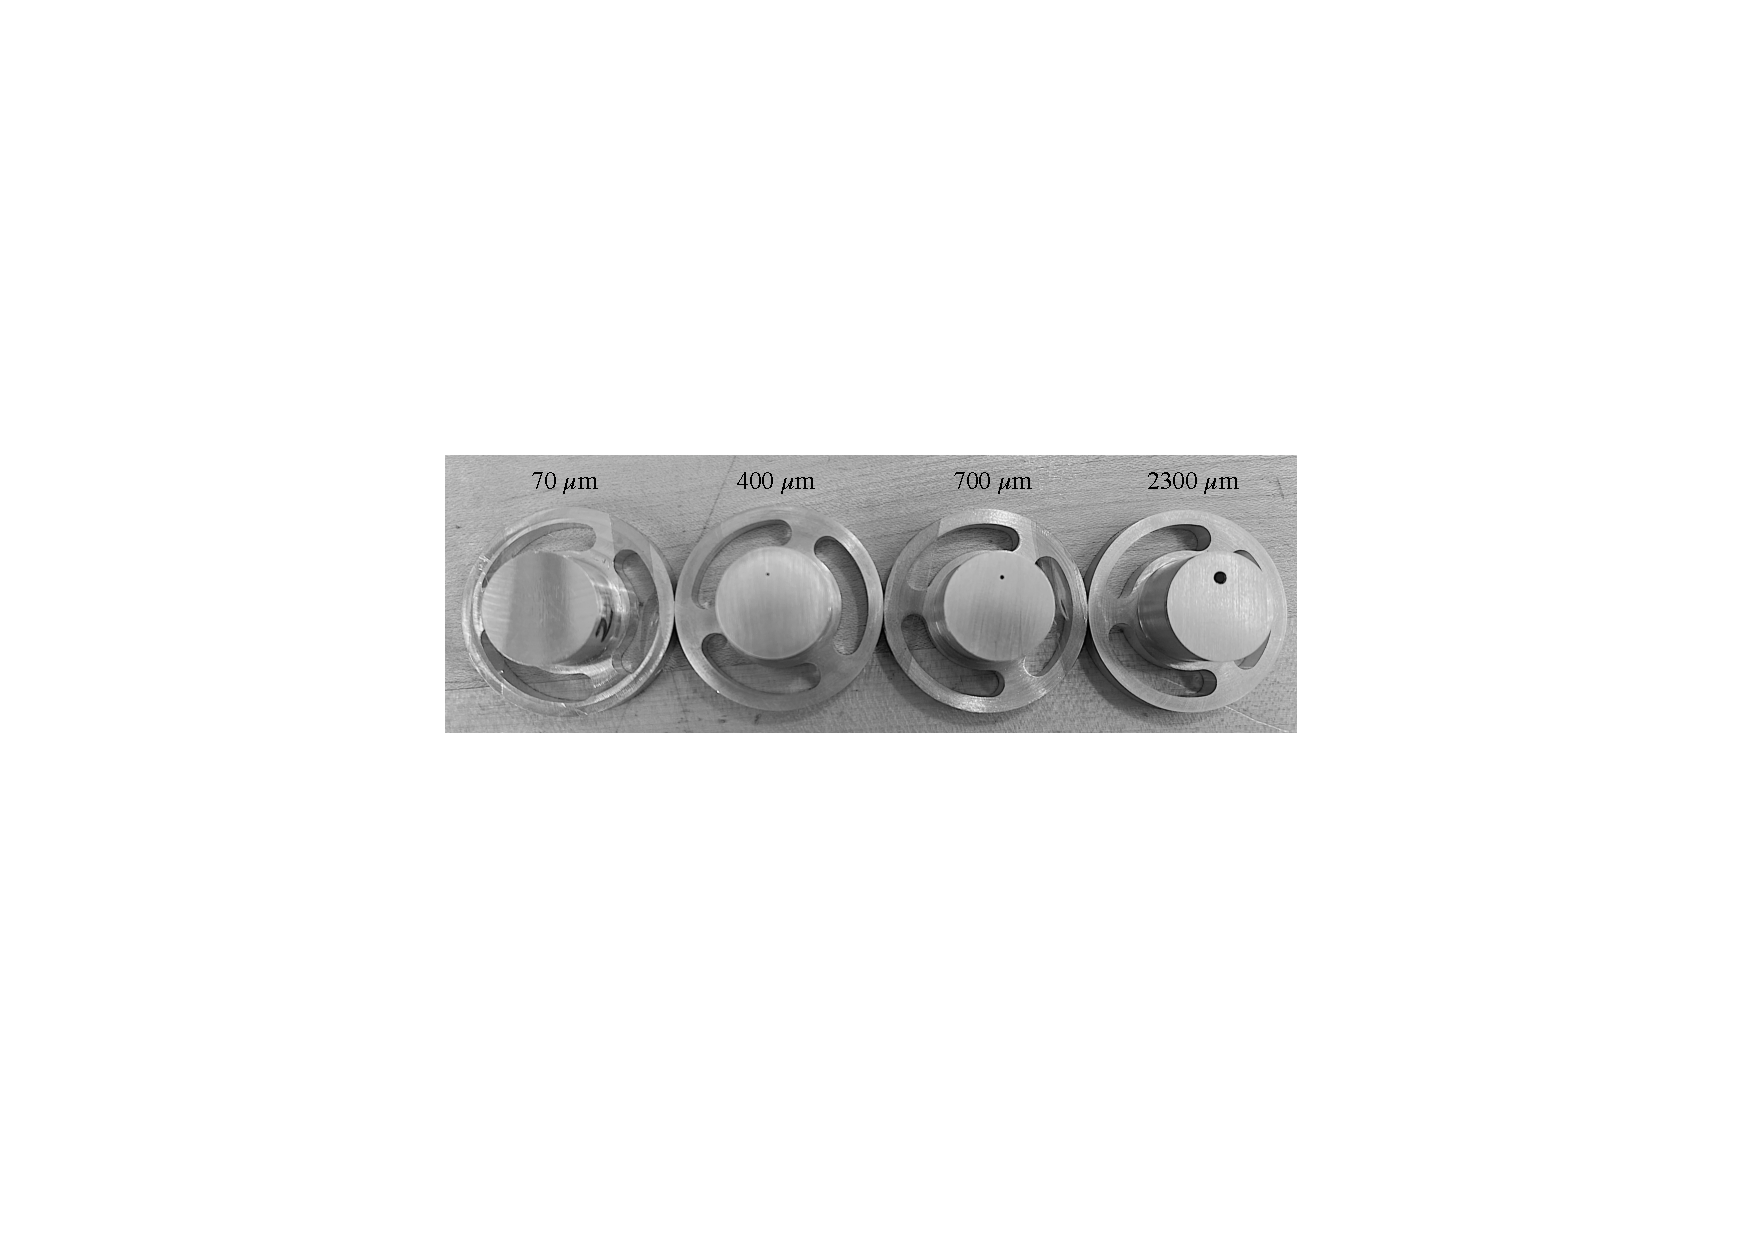
\includegraphics[width=0.7\textwidth]{pinholes.pdf}
  \end{figure}

  \begin{itemize}
    \centering
        \item Testing pinhole diameters of $d=$ 2300, 700, 400 $\mu$m
        \item Corresponds to $d^+ \approx$ 85, 93, 108
        \item Under the frozen turbulence assumption, these sit around $T^+\sim 10$
    \end{itemize}
\end{frame}

\begin{frame}
  \frametitle{Pinhole spacings}

  \begin{columns}
    \begin{column}{0.3\textwidth}
      \begin{figure}
        \centering
        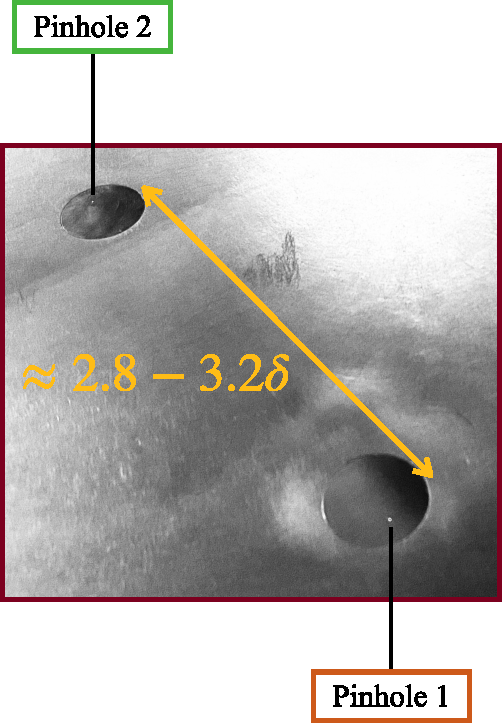
\includegraphics[width=\textwidth]{pinhole_spacing.pdf}
      \end{figure}
    \end{column}
    \begin{column}{0.5\textwidth}
      \begin{itemize}
        \item We have two-point measurements at two streamwise spacings: $3.2\delta$ and $2.8\delta$
        \item Herein, we refer to these as `far' and `close' spacings
        \item The spectra are plotted in voltage and haven't yet been converted to pressure
      \end{itemize}
    \end{column}
  \end{columns}
\end{frame}


\begin{frame}
  \frametitle{Measurements are very sensitive to their fitting}
  \begin{figure}
  \centering
    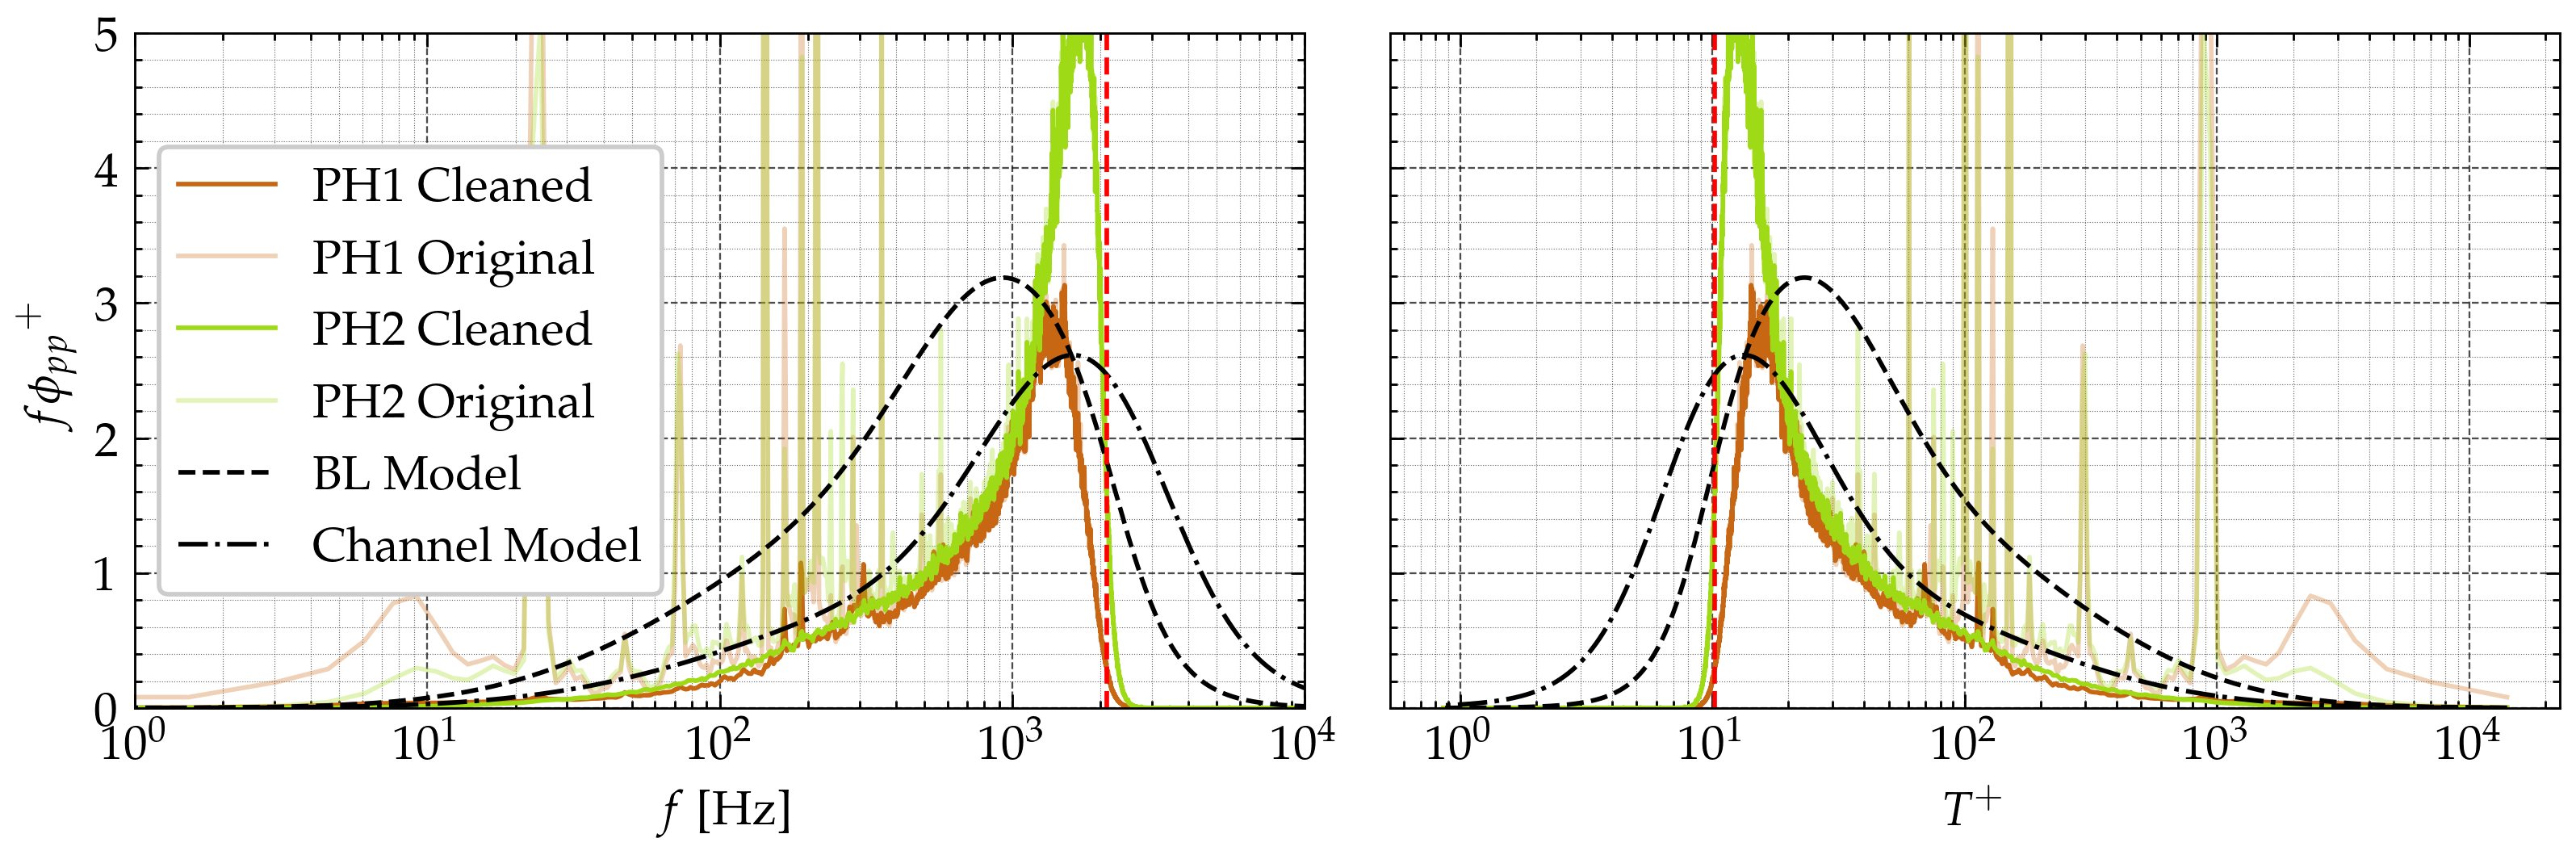
\includegraphics[width=0.7\textwidth]{remount_test/original_cleaned.png}
    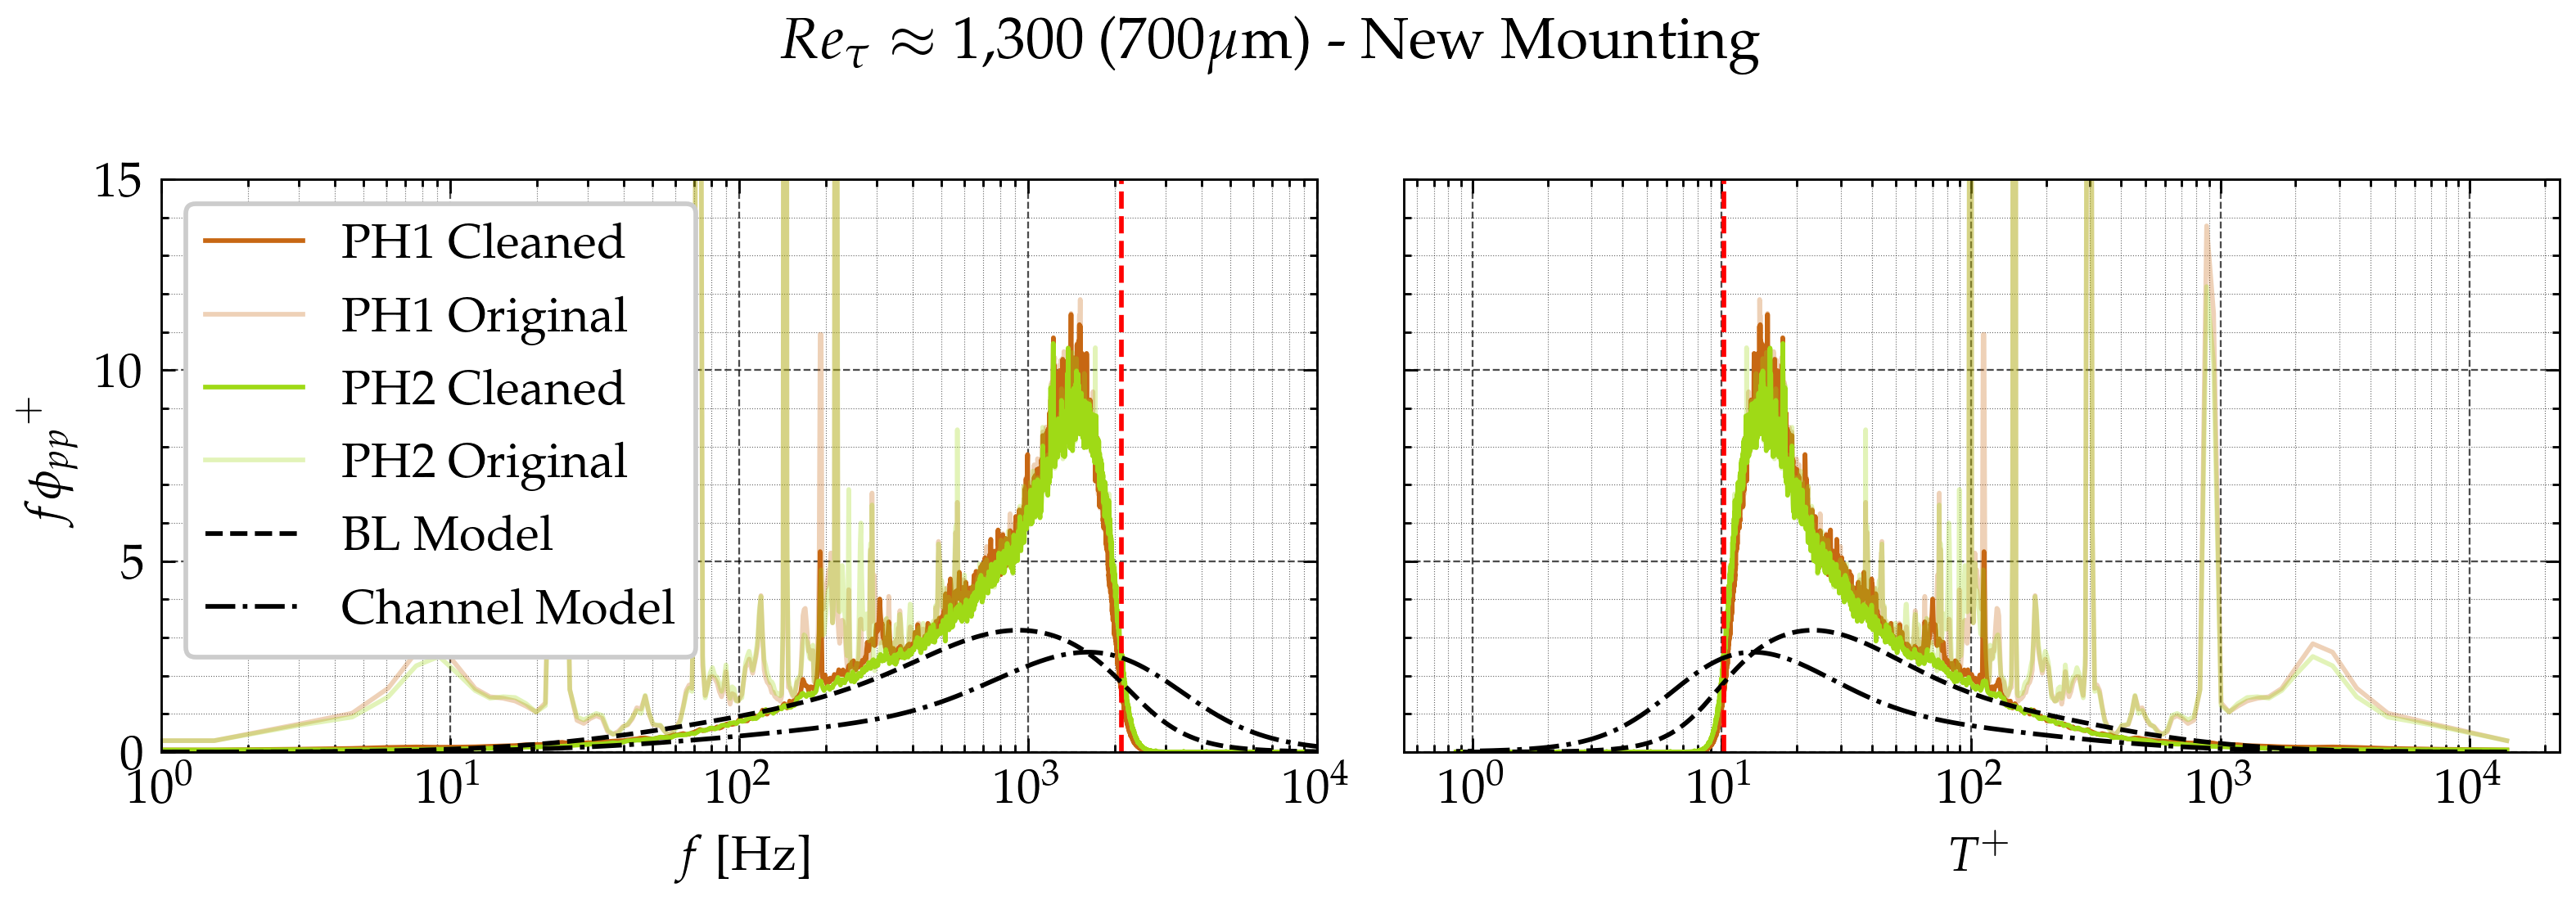
\includegraphics[width=0.7\textwidth]{remount_test/new_mount_cleaned.png}
  \end{figure}

\end{frame}

\section{New measurements}
\begin{frame}
  \centering
  \vfill
  {\Huge\bfseries \textcolor{cardinalred}{New measurements}}
  \vfill
\end{frame}


\begin{frame}
  \frametitle{New measurements [Pa]: $Re_\tau\approx$ 1,300 ($d=$700 $\mu$m)}
  \begin{figure}
    \centering
    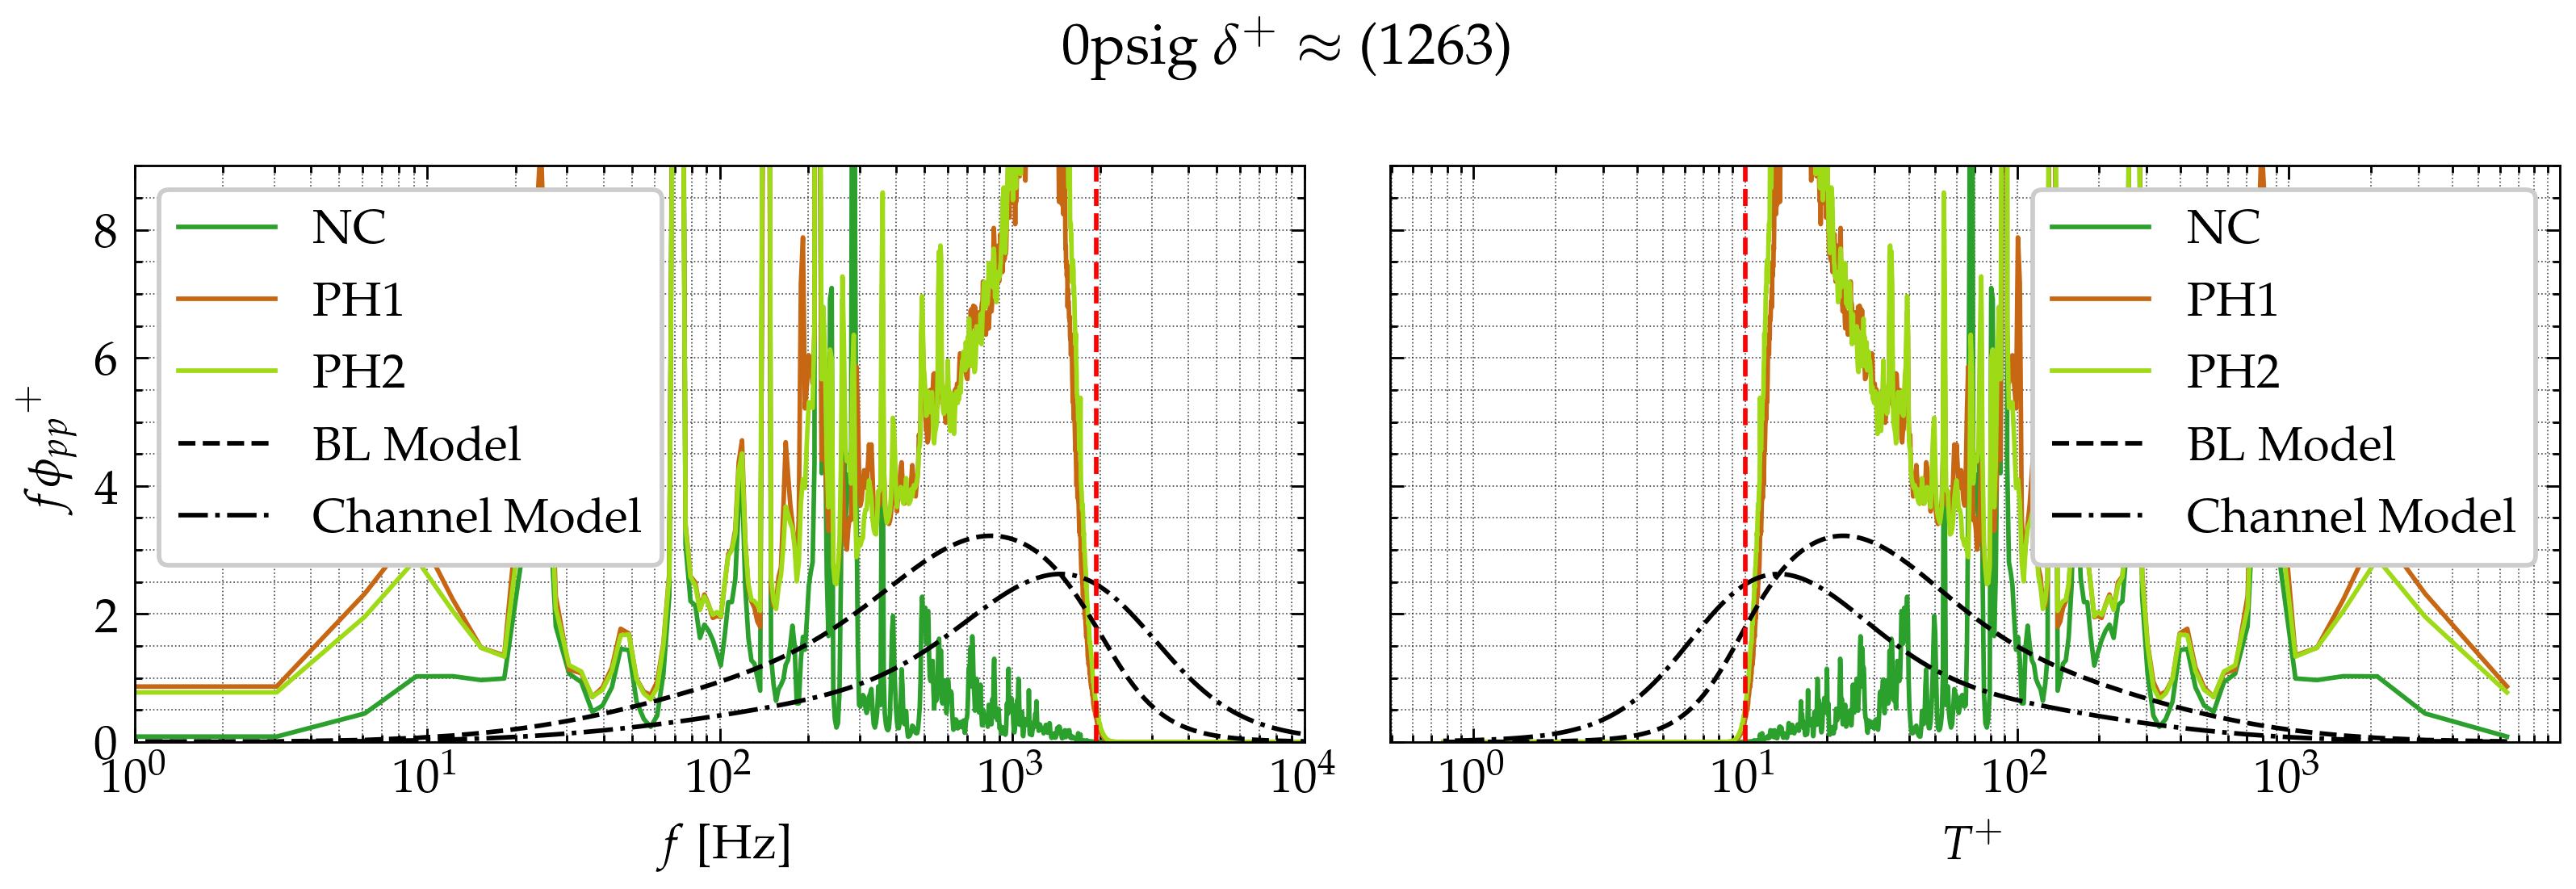
\includegraphics[width=0.9\textwidth]{final/0psig.png}
  \end{figure}
\end{frame}

\begin{frame}
  \frametitle{New measurements [Pa]: $Re_\tau \approx$ 4,700 ($d=$700 $\mu$m)}
  \begin{figure}
    \centering
    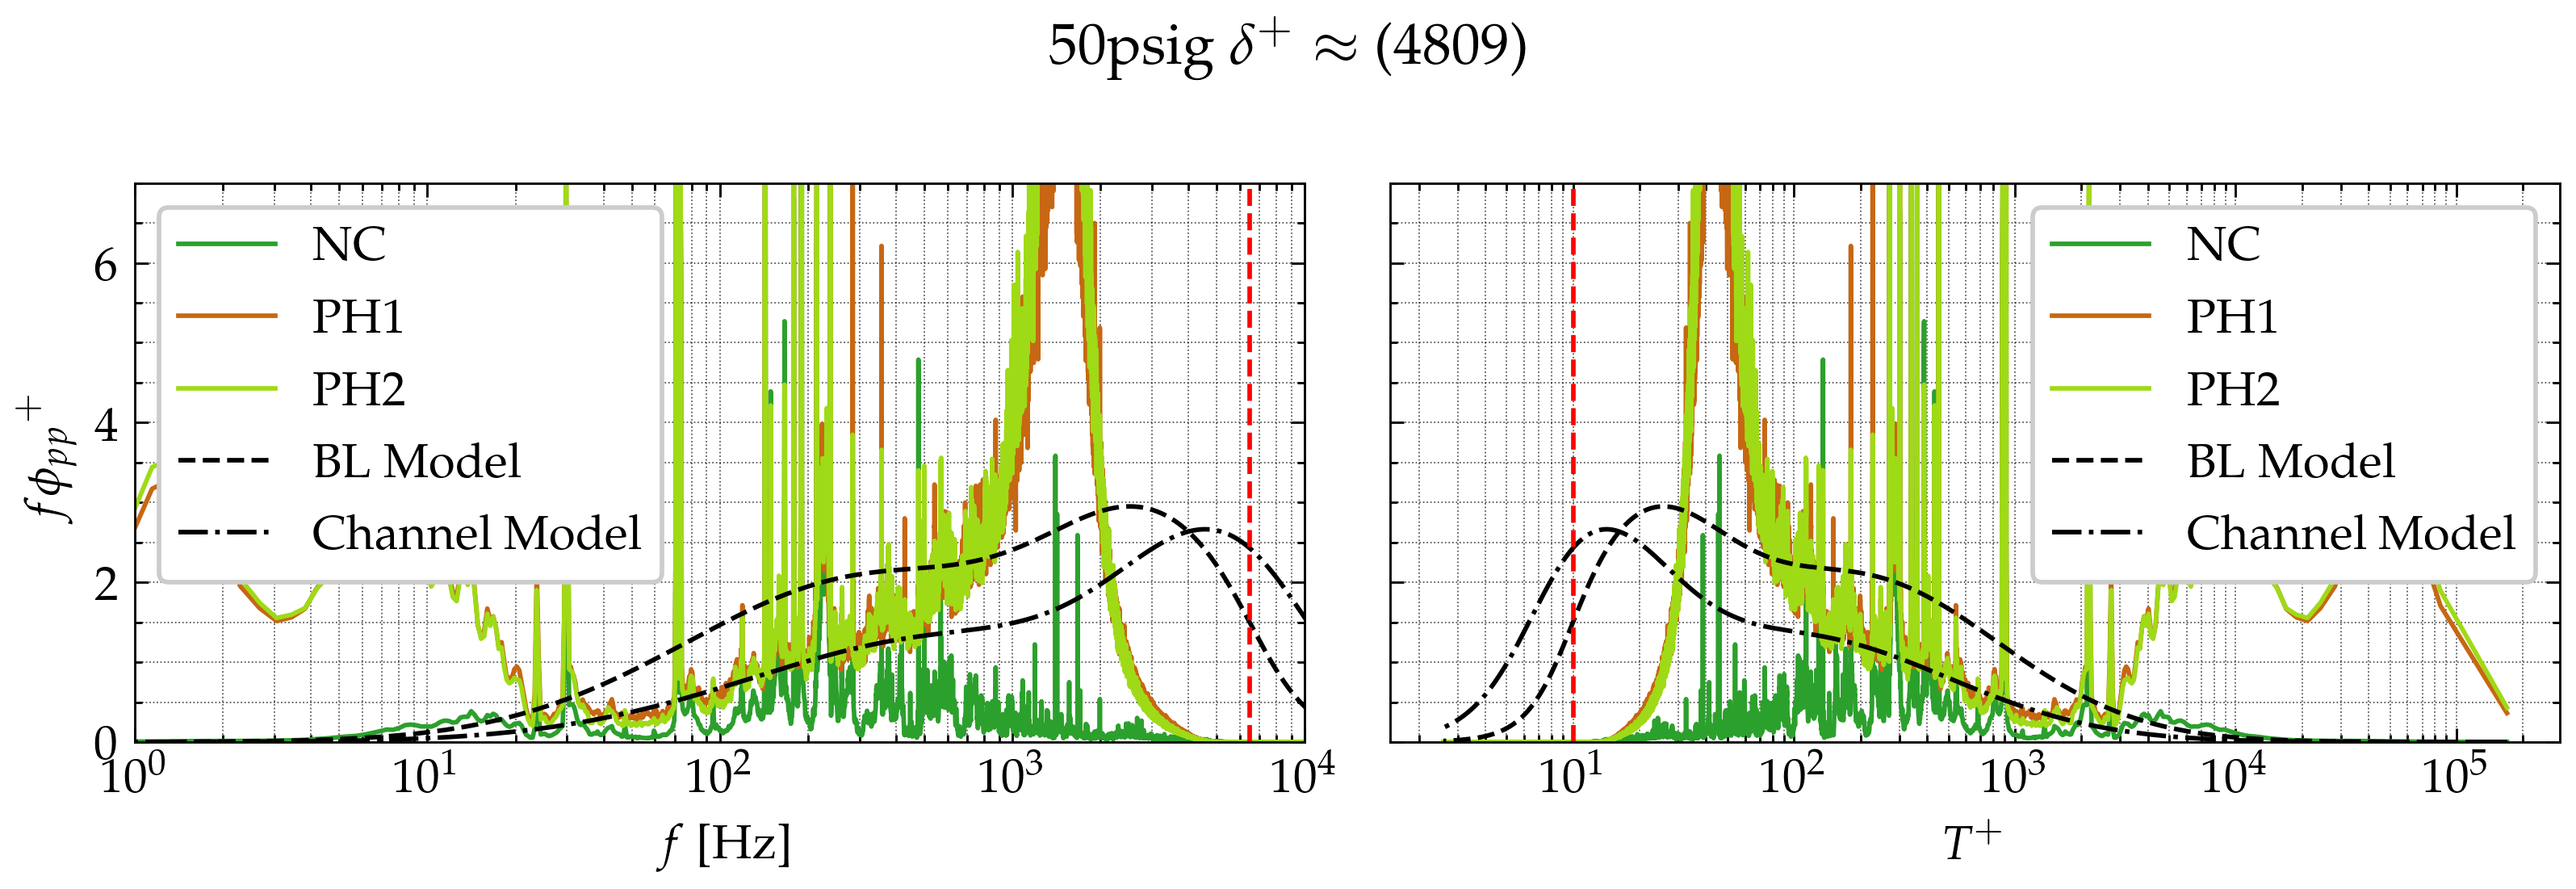
\includegraphics[width=0.9\textwidth]{final/50psig.png}
  \end{figure}
\end{frame}

\begin{frame}
  \frametitle{New measurements [Pa]: $Re_\tau \approx$ 9,500 ($d=$700 $\mu$m)}
  \begin{figure}
      \centering
      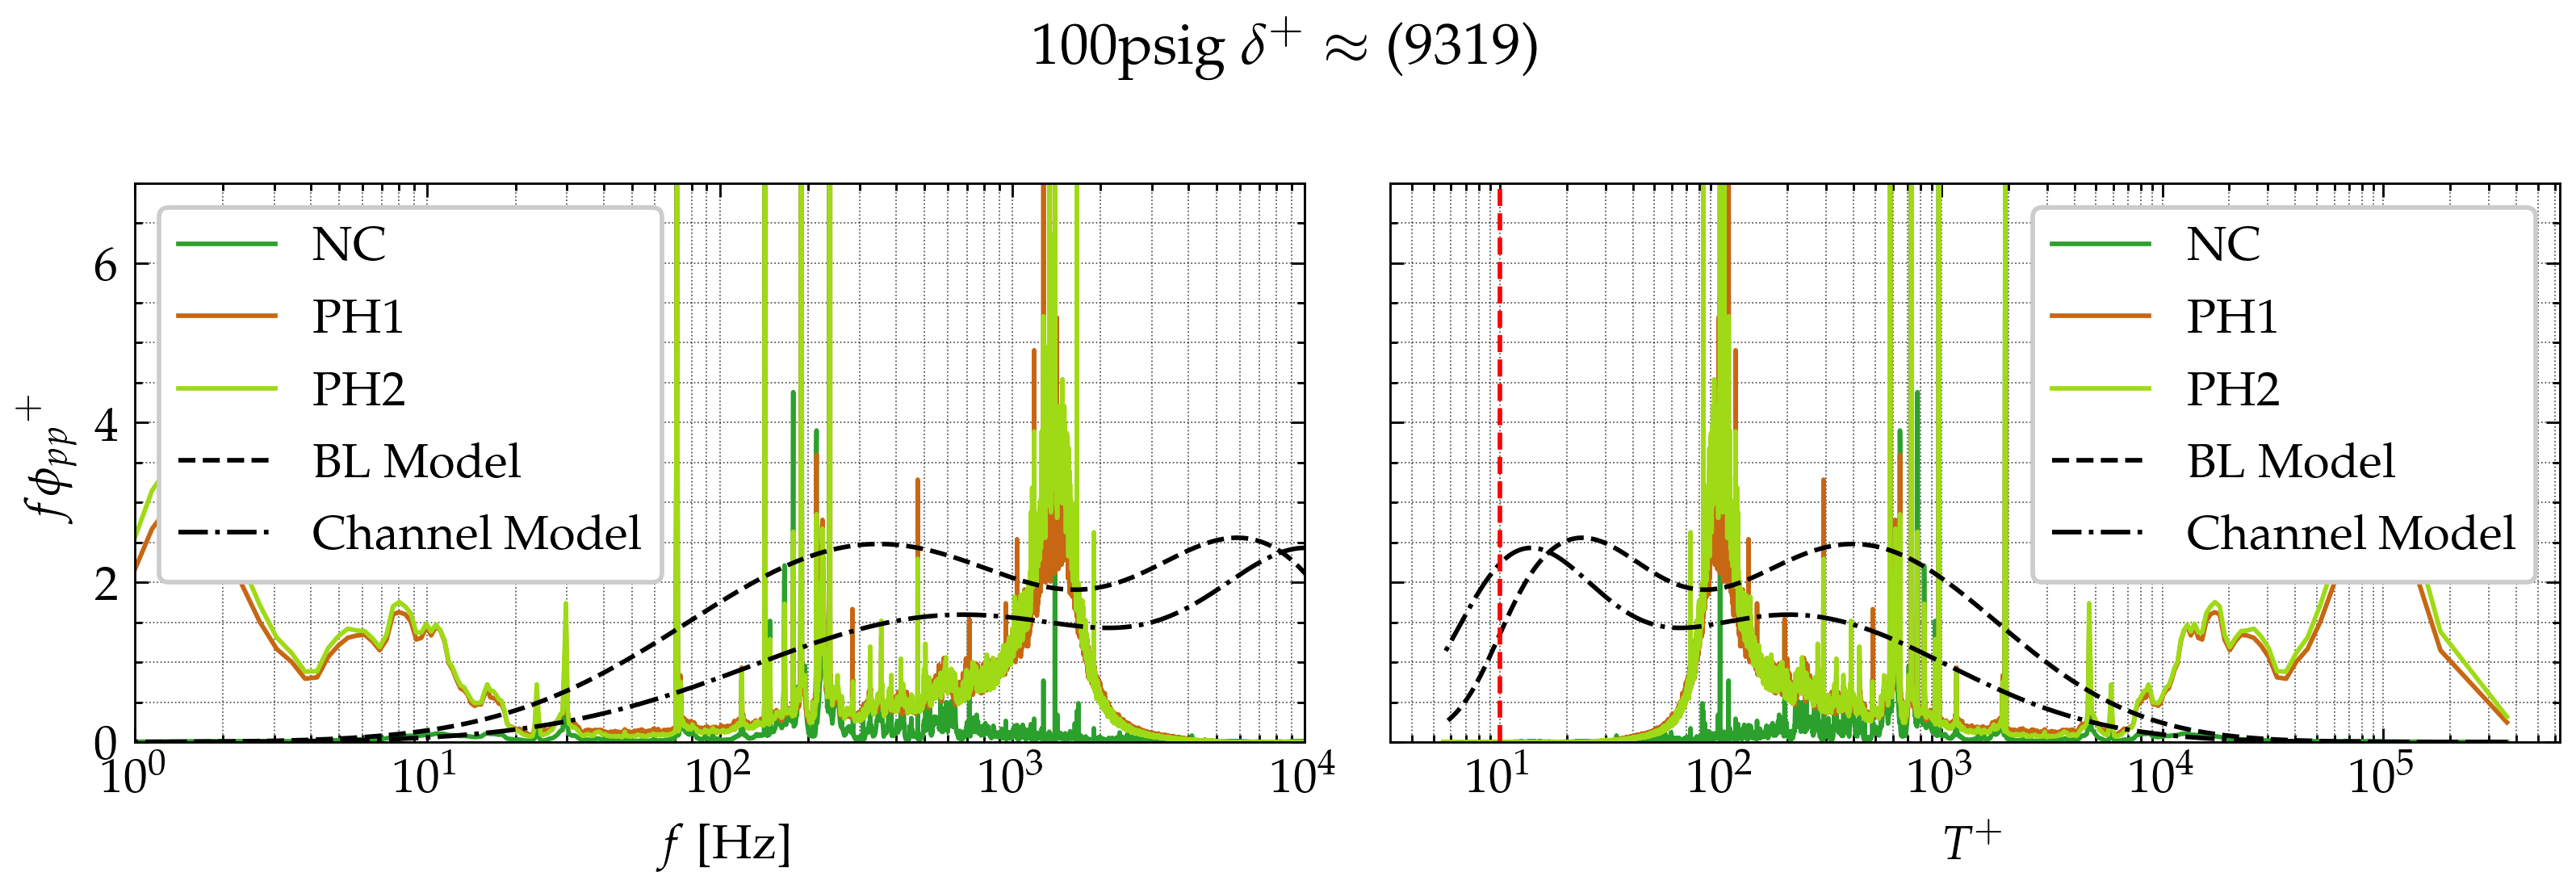
\includegraphics[width=0.9\textwidth]{final/100psig.png}
  \end{figure}
\end{frame}

\begin{frame}
  \frametitle{FS noise rejected}
  \begin{figure}
      \centering
      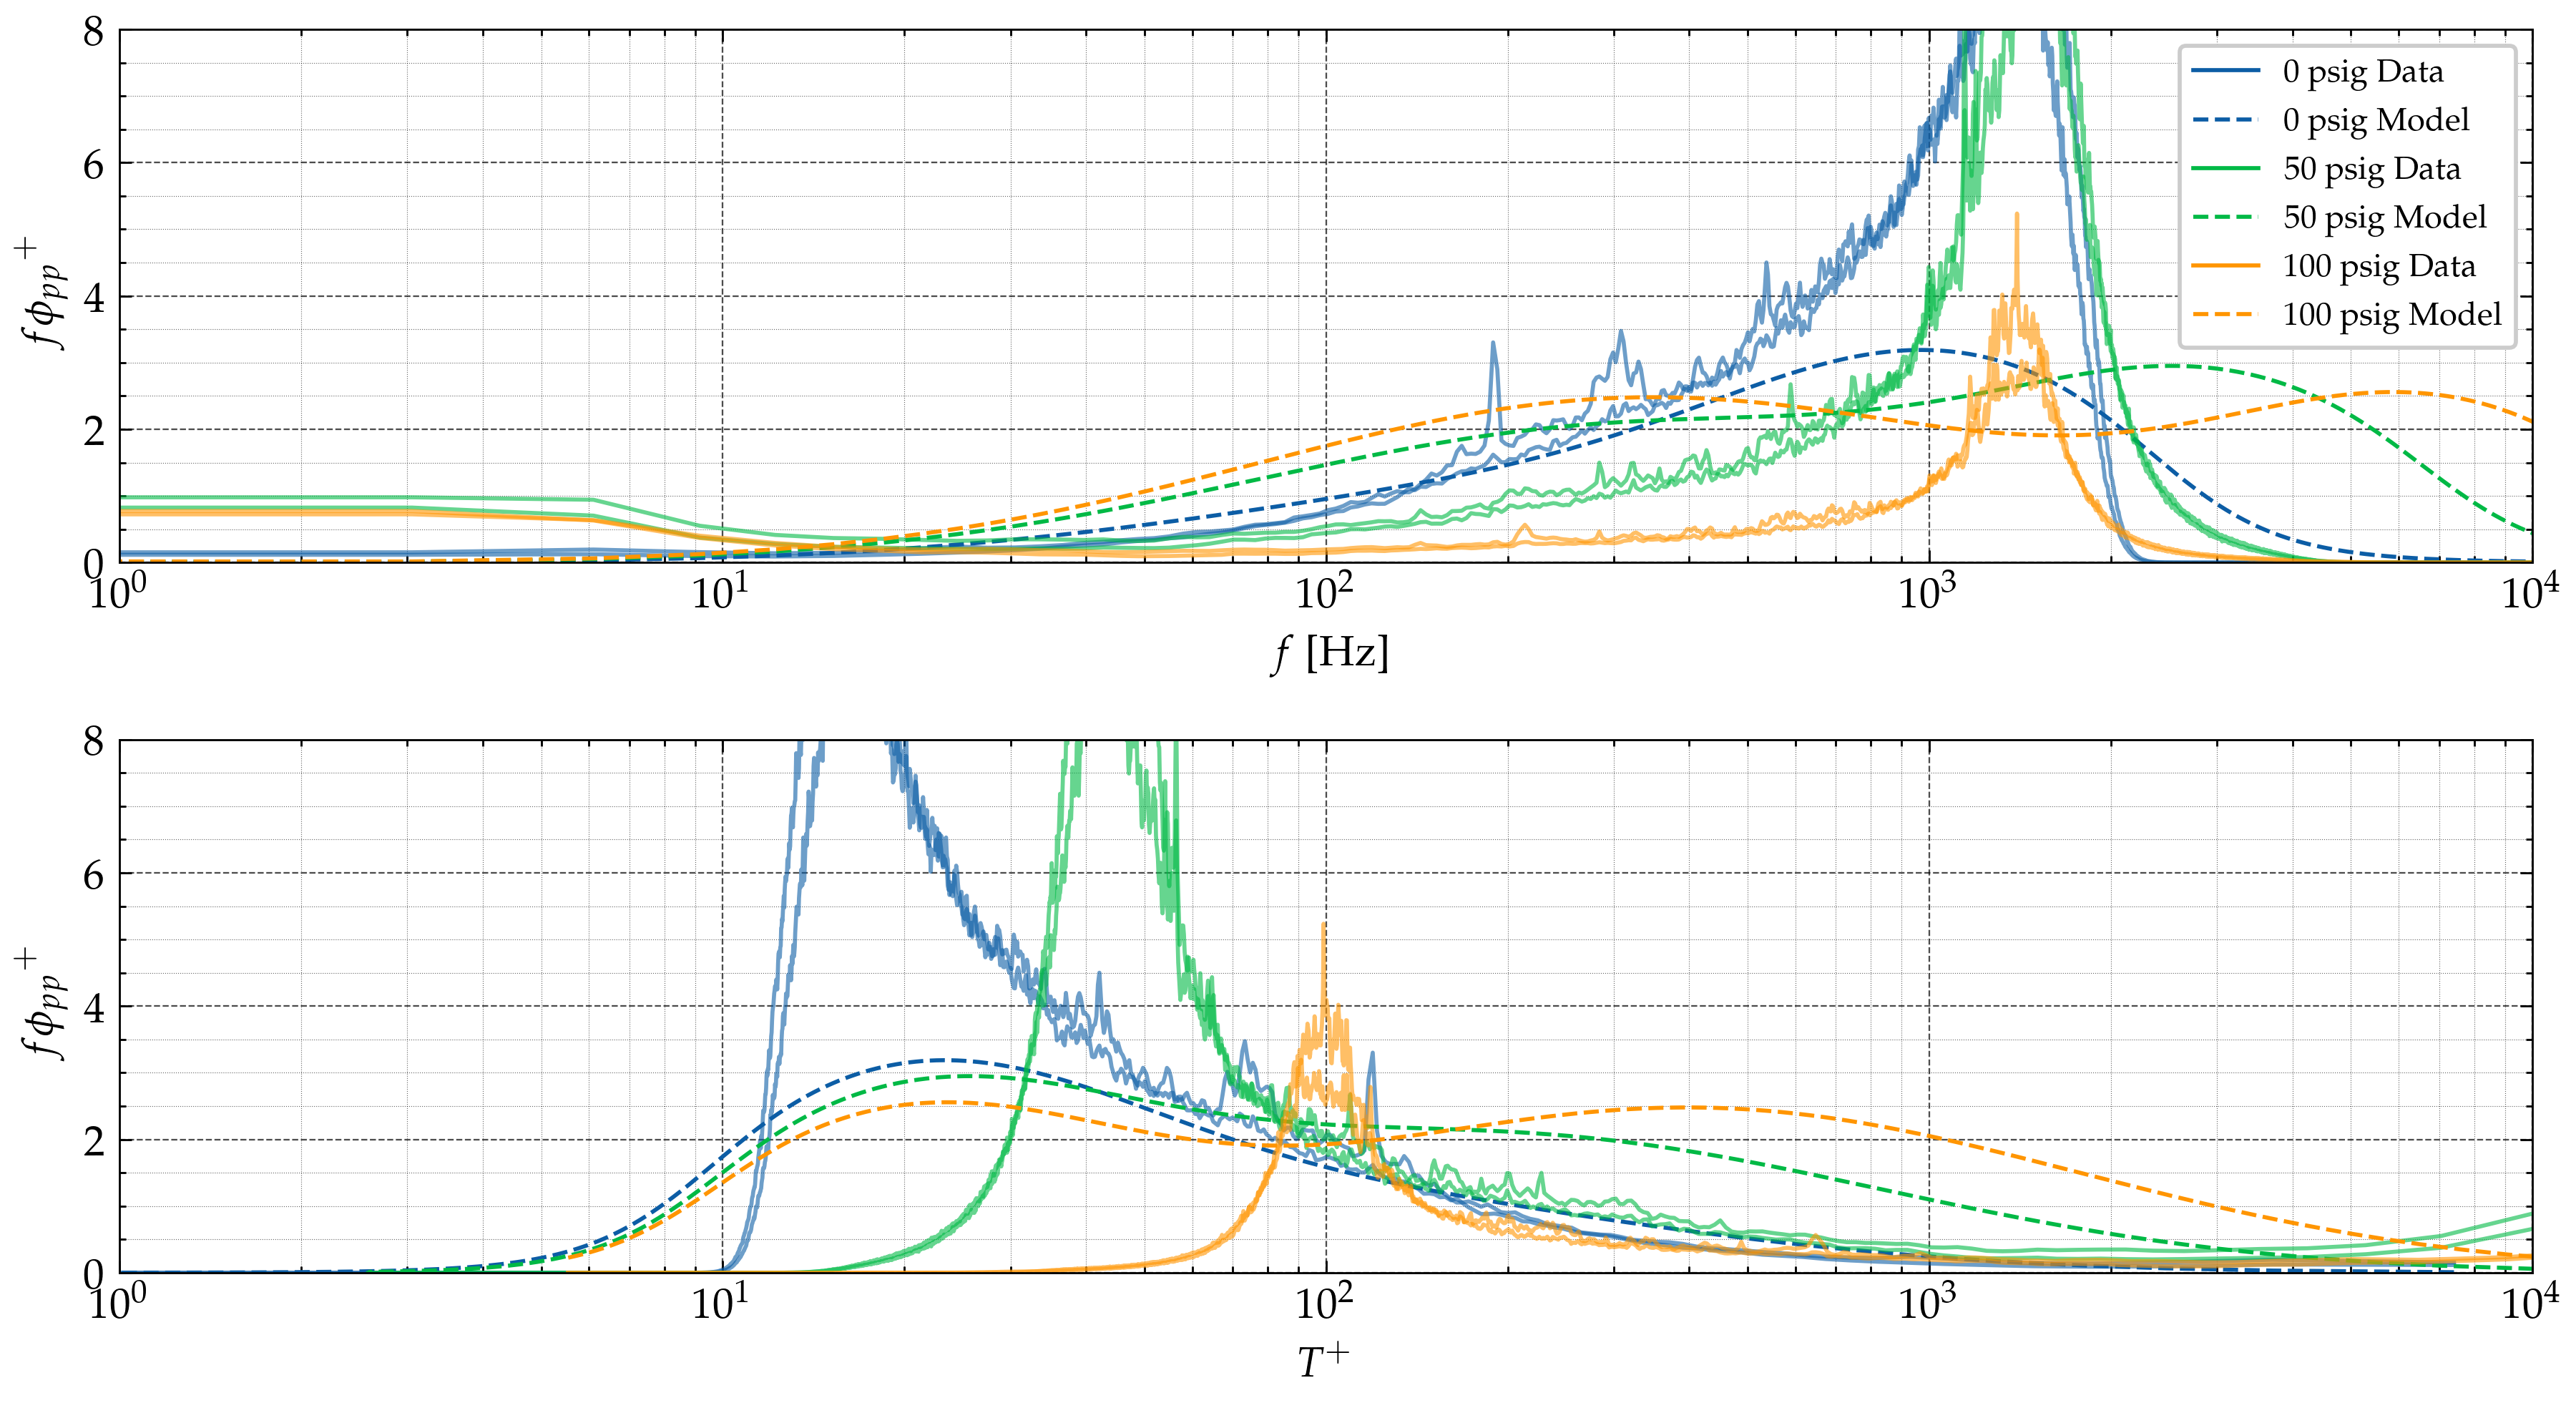
\includegraphics[width=0.9\textwidth]{final/spectra_comparison.png}
  \end{figure}
\end{frame}



\section{Best estimate}
\begin{frame}
  \centering
  \vfill
  {\Huge\bfseries \textcolor{cardinalred}{Best estimate}}
  \vfill
\end{frame}

\begin{frame}
  \frametitle{Mapping the data to the model gives us an idea of what the TFs \emph{should} be (- - lines are currently measured)}
  \begin{figure}
      \centering
      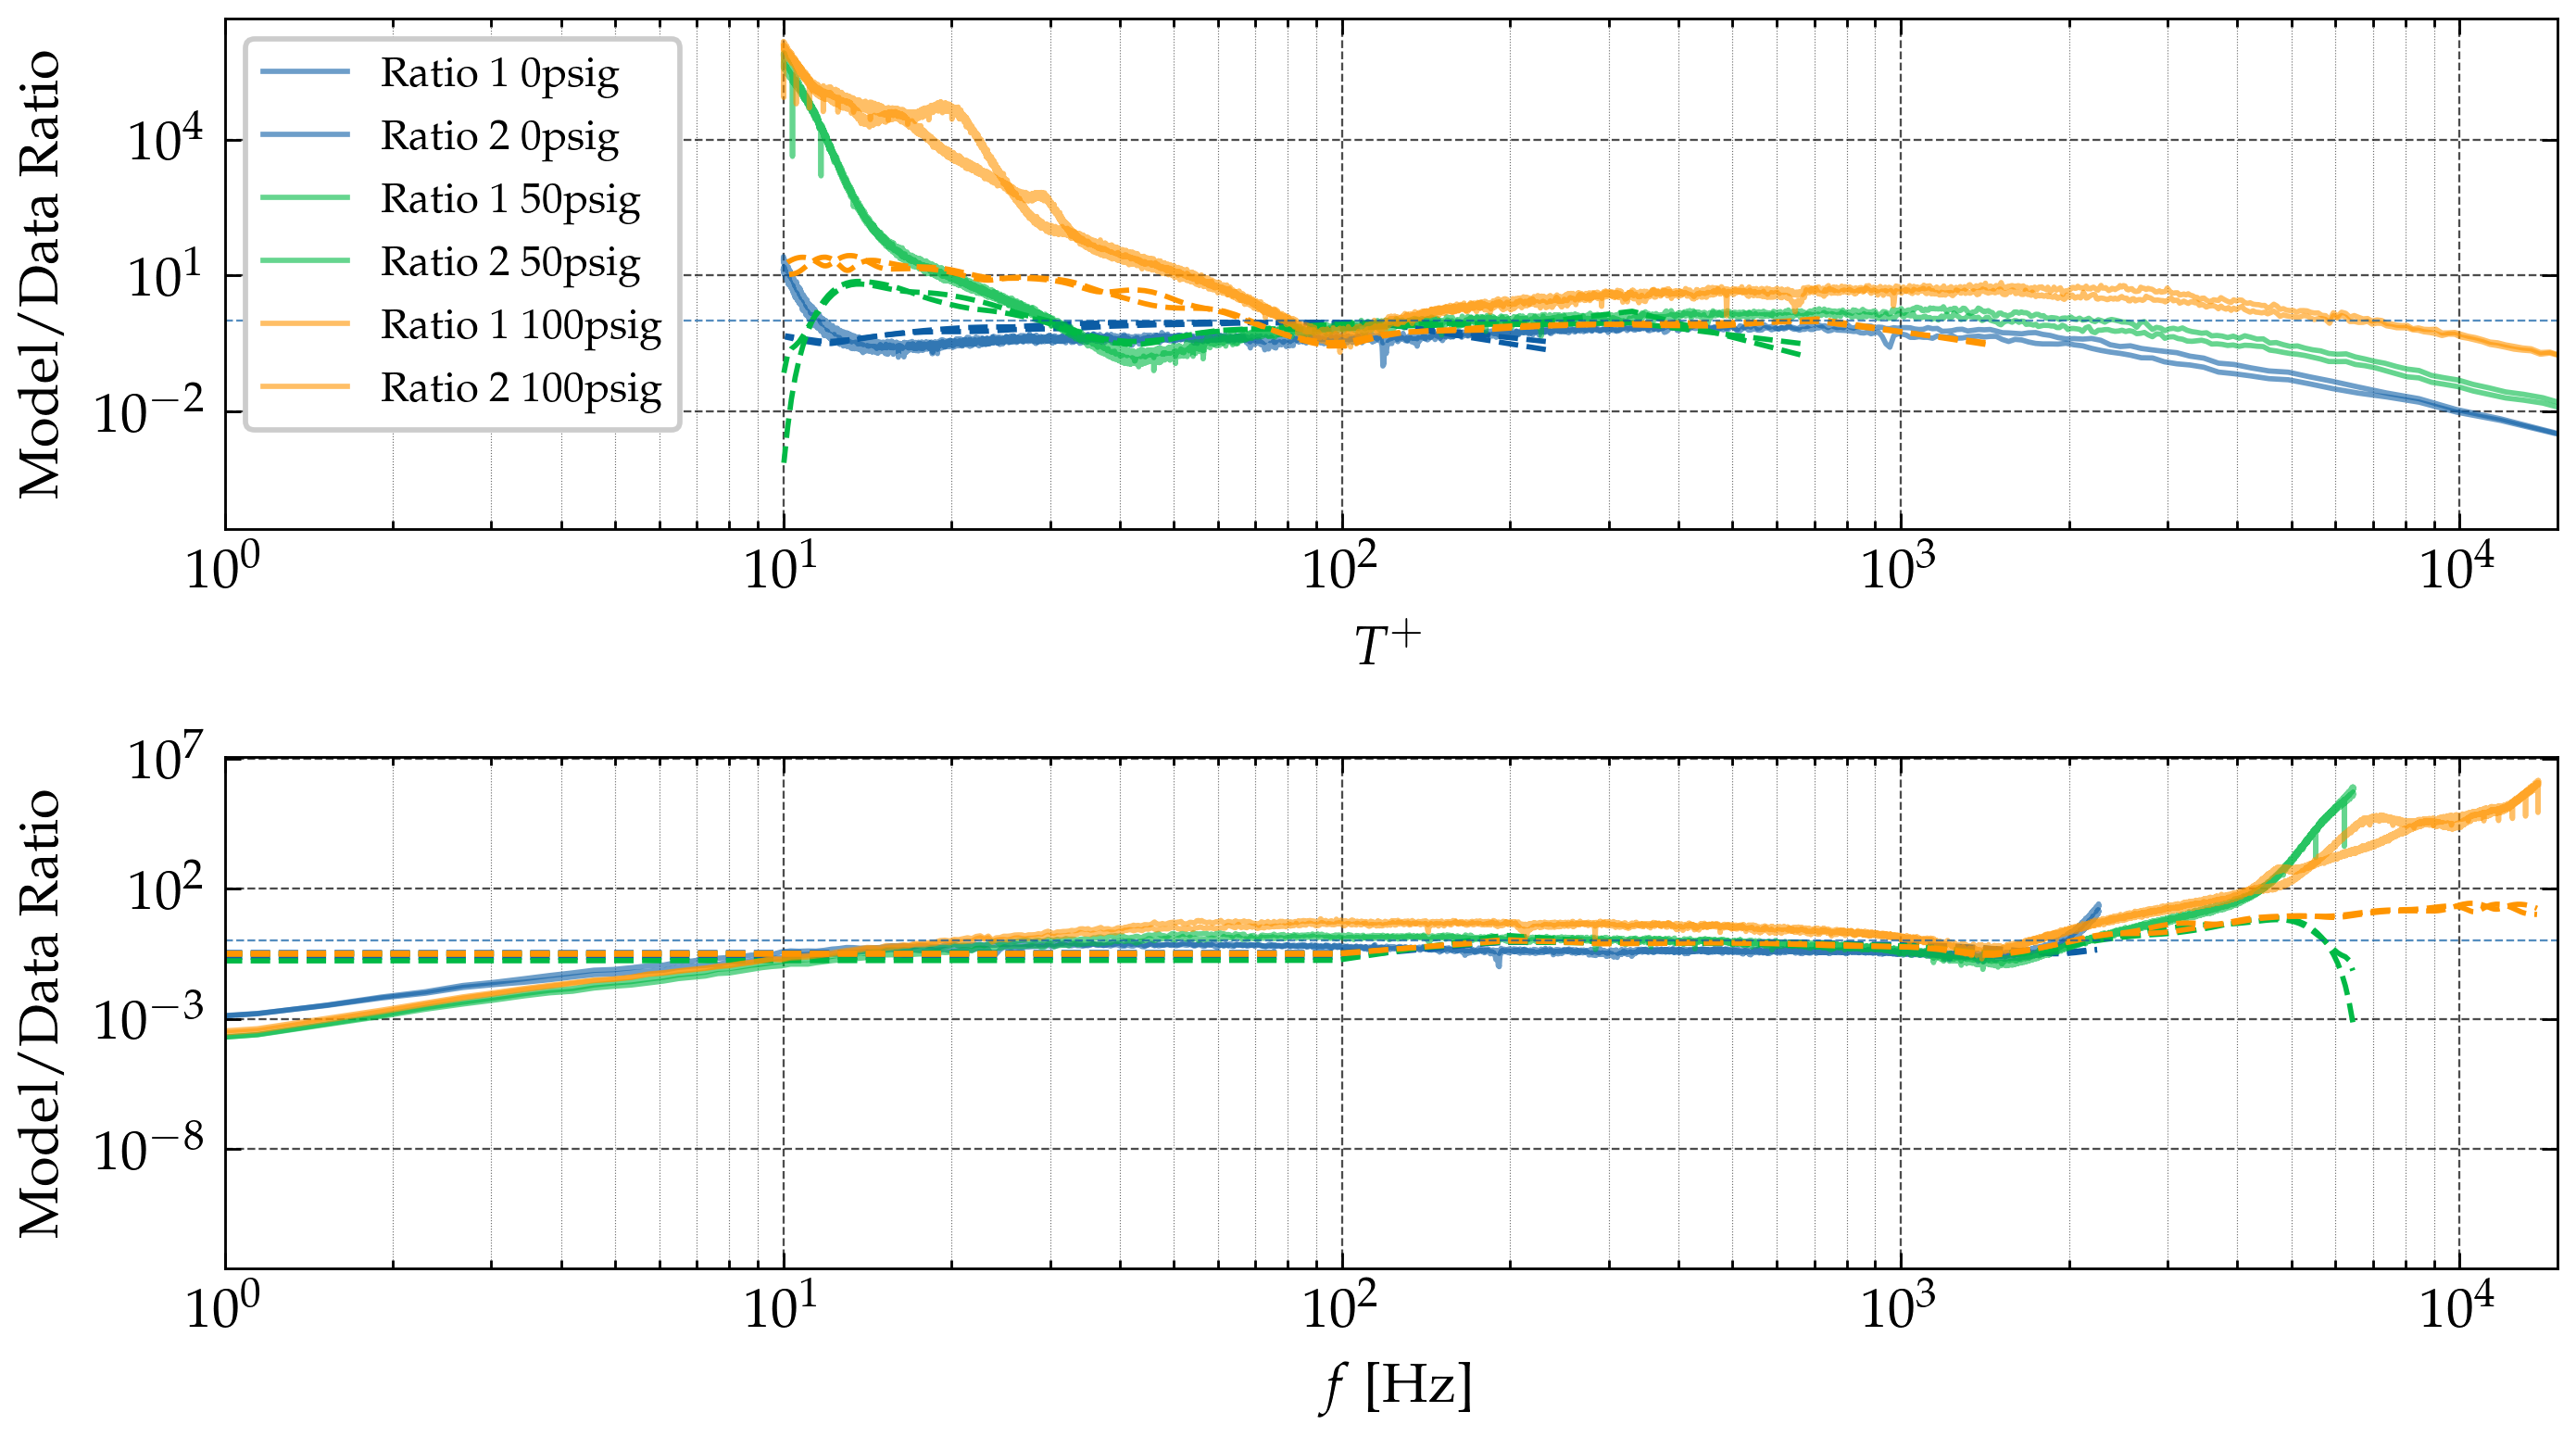
\includegraphics[width=0.8\textwidth]{final/required_transfer_functions.png}
  \end{figure}
\end{frame}

\begin{frame}
  \frametitle{We need more transfer function data, our current best estimate:}
  \begin{figure}
      \centering
      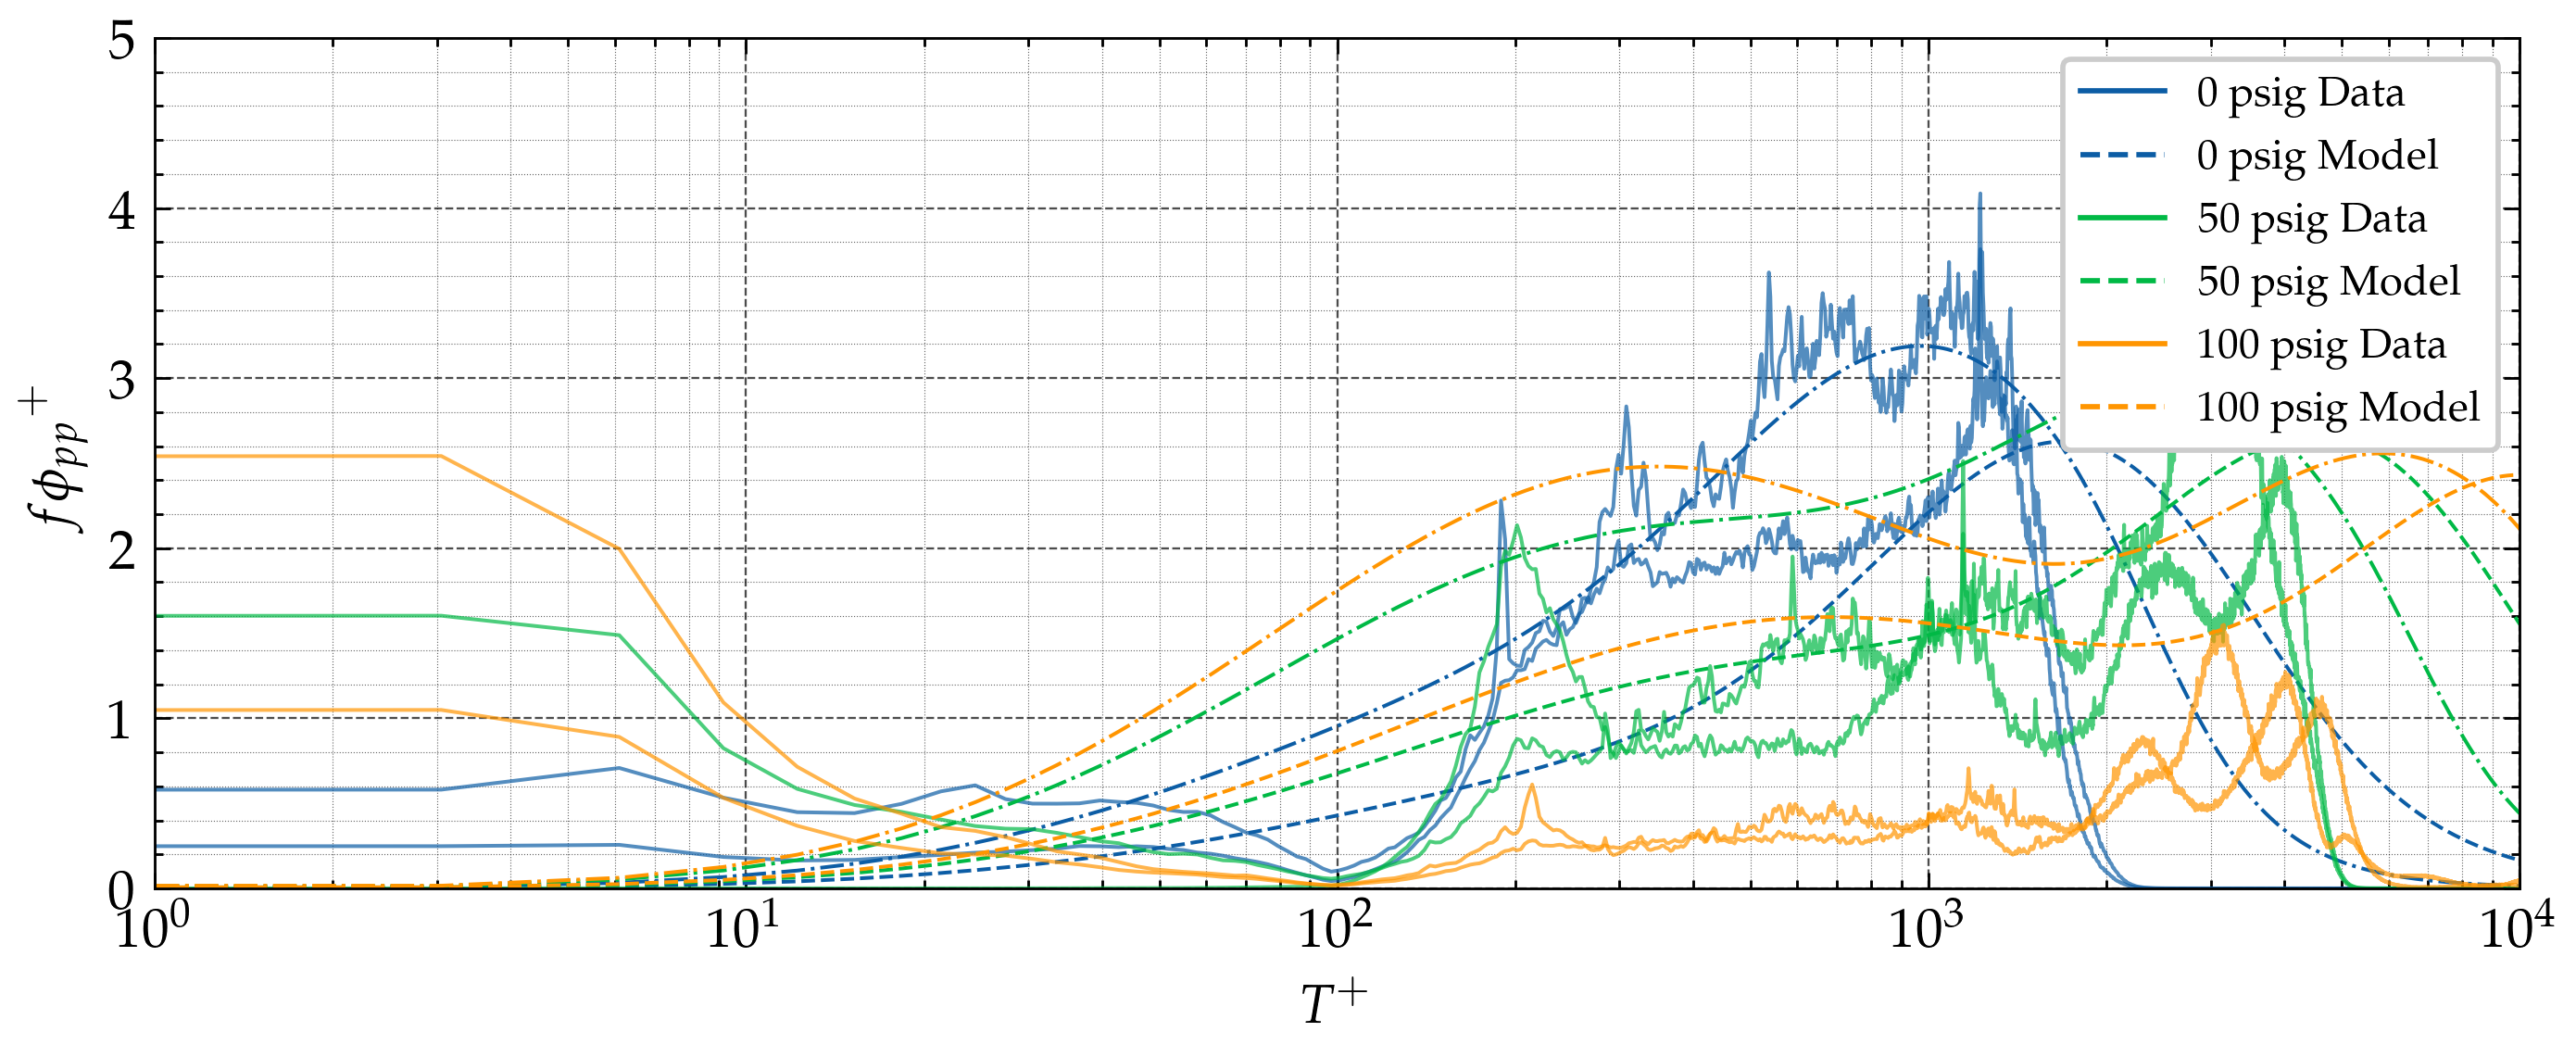
\includegraphics[width=0.9\textwidth]{final/spectra_comparison_tf.png}
  \end{figure}
\end{frame}


\end{document}
